\section{Channel Encoding}
\begin{definition}
DMC(Discrete memoryless channel): Input alphabet $\mathcal{X}$, output alphabet $\mathcal{Y}$.
\end{definition}
\begin{figure}[htbp]
    \centering
    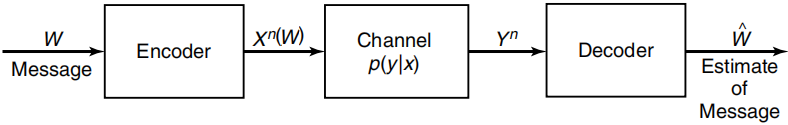
\includegraphics[width=\textwidth]{./figures/chapter5/communication_system.png}
\end{figure}
A $(M, n)$ code consists of (here $M$ takes $2^{nR}$, $M$是index range, $n$是block length): \\
1. $W\in[1:2^{nR}]$, Uniformly distributed in $[1:2^{nR}]$ \\
2. Encoder: $X^n=f(W)$, $[1:2^{nR}]\to\mathcal{X}^n$ \\
3. Channel: $Y^n=p(Y^n|X^n)$ \\
4. Decoder: $\hat{W}=g(Y^n), \mathcal{Y}^n\to[1:2^{nR}]$

Some definitions: \\
1. error probability: $\lambda(i)=\Pr\left[\hat{W}\neq i | W=i\right]$ \\
2. $\lambda^{(n)}=\max\limits_{i\in[1,w^{nR}]}\lambda(i)$ \\
3. average error probability: $p_e^{(n)}=\dfrac{1}{2^{nR}}\sum\limits_{i=1}^{2^{nR}} \lambda(i)$

(\textcolor{red}{和$p_e^{(n)}\to 0$相比, $\lambda(i)\to 0$ constrain更强}) \\
4. The rate $R$ of an $(M,n)$ code is $R=\dfrac{\log M}{n}$ \textcolor{red}{bits per transmission}

当$M=2^{nR}$时理解: 信道编码把信源index(W)映射到$X^n$, 用$n$次传输传送$W$. 因为$W$从$[1,\ldots,M]$中均匀采样, 在无损传输的条件下($p_e^{(n)}\to 0$), 平均每次用信道发送的bit数为 $\dfrac{H(W)}{n}=\dfrac{\log M}{n}=\dfrac{\log 2^{nR}}{n}=R$. \\
5. $R$ is achievable if $\exists (n,R)$, s.t. $p_e^{(n)}\to 0$. \\
6. The capacity of a channel $C$ is the maximum(supremum) of all achievable rate $R$. \\
7. Codebook: $\mathcal{C}=\left\{X^n(1),X^n(2)\ldots,X^n(2^{nR})\right\}$ ($X^n(i)$: 长度为$n$的第$i$个序列)

Memoryless: distribution of outputs depends only on the input of that time. 当前输出只与当前输入有关
$$\textcolor{red}{p(y_k|x_k,y_{k-1})=p(y_k|x_k)\Rightarrow p(y^n|x^n)=\prod\limits_{k=1}^np(y_k|x_k)}$$

\textcolor{blue}{常数与任何变量都独立, $X$ is deterministic, $I(X;Y)=0$.}

\begin{figure}[htbp]
    \centering
    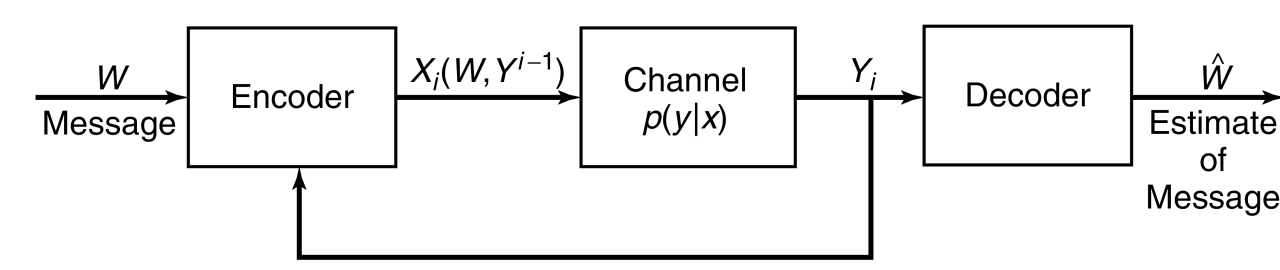
\includegraphics[width=\textwidth]{./figures/chapter5/feedback_channel.png}
\end{figure}


DMC with feedback 和没有feedback相比, 不会增加信道容量
\begin{align*}
p(y^n|x^n) &= \prod\limits_{k=1}^np(y_k|x^n,y_1,\ldots,y_{k-1}) \\
X_i &= f(W,Y_1,\ldots,Y_{i-1})
\end{align*}